\scanpage{174}

$\operatorname{Spec}\mathbf Z$

\figure{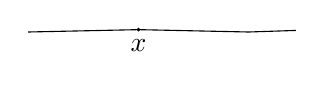
\begin{tikzpicture}\draw (0,0)--(1.4,0.03)--(2.8,0)--(3.4,0.02);\fill (1.4,0.03) circle (0.025);\node[below] at (1.4,0.03) {$x$};\end{tikzpicture}}

\[
i_x^!(M)=\unsure{R}i_x^*(M)(-1)[-2]
\]

\diagram{\begin{tikzcd}[column sep=small]
\cdots \arrow[r,no head]&H^{i-2}(x,i_x^*(M)(-1))\arrow[r]&H^i(X,M)\arrow[r,no head]&H^i(U,M)\arrow[r,no head]&H^{i-1}(x,i_x^*(M)(-1))\arrow[r]&\cdots
\end{tikzcd}}

\[
M=\underset{\sim}{\mathbf Q}(n)
\]
\deleted{$\unsure{H^i|H^2}$}
\[
\left\{\begin{aligned}
&i\neq1,2,3\qquad H^i(X,M)\xrightarrow{\sim}H^i(U,M)\\[1em]
&0\longrightarrow H^1(X,M)\longrightarrow H^1(U,M)\longrightarrow H^0(S,i_x^*(M)(-1))\longrightarrow H^2(X,M)\\[1em]
&\hspace{3em}\longrightarrow H^2(U,M)\longrightarrow H^1(S,i_x^*(M)(-1))\longrightarrow H^3(X,M)\\[1em]
&\hspace{3em}\longrightarrow\underset{=\,0?}{H^3(U,M)}\longrightarrow0
\end{aligned}\right.
\]
\margin{\unsure{pas de miracle}, car si $i\geq4$, les deux \unsure{mbs} doivent être $=0$.}

\[
M=\deleted{\unsure{\mathbf Z_l}}\mathbf Q_{\deleted{\unsure{l}}}(n),\qquad i_x^*(M)\unsure{(-1)|H_l}=\mathbf Q(n-1)_S
\]

\uline{Si $n\neq1$}\qquad $H^i(X,\mathbf Q(n))\xrightarrow{\sim}H^i(U,\mathbf Q(n))$\qquad\uline{tout $i$}
\margin{[\unsure{est-on|est-ce} nul ??]}

Si $n=1$
\diagram{\begin{tikzcd}[column sep=small]
0\arrow[r,no head]&H^1(X,\mathbf Q(1))\arrow[r]&H^1(U,\mathbf Q(1))\arrow[r]&\mathbf Q^S\arrow[r]&H^2(X,\mathbf Q(1))\arrow[r]&{}\\
{}&{}&H^2(U,\mathbf Q(1))\arrow[r]&\mathbf Q^S\arrow[r]&H^3(X,\mathbf Q(1))\arrow[r]&0
\end{tikzcd}}

$H^i(X,\mathbf Q(1))=0$ sauf pour $i=3$, \unsure{où on trouve} $\mathbf Q$ !

\margin{173}
